

\documentclass[twocolumn]{svjour3}       
\journalname{VLDBJ}

%% Font related stuff
%\usepackage{times} 
\usepackage{amsmath} 
\usepackage{amsfonts} 
\usepackage{amssymb} 
%\usepackage{amsthm} 
\usepackage{bold-extra} 
\usepackage[T1]{fontenc} % prettier curly braces in tt mode
\usepackage[scaled]{beramono}
% prettier emptyset
\let\oldemptyset\emptyset
\let\emptyset\varnothing
\DeclareMathOperator{\dist}{dist}

%% Algorithms
\usepackage{listings}
\usepackage[ruled,vlined]{algorithm2e}
\DontPrintSemicolon
\renewcommand{\CommentSty}[1]{\textnormal{#1}}
\SetKwComment{tcp}{$\triangleright$ }{}
\SetVlineSkip{0cm}
\SetAlgoSkip{}


%% others
\usepackage{alltt}
\usepackage{color}
\usepackage{url}
\usepackage[pdftex]{hyperref}
\usepackage{graphicx}
\usepackage{multirow}
\usepackage{blkarray}
\usepackage{balance}
\usepackage{mdframed}

%\usepackage{enumitem}
%\setlist{nolistsep}
%\usepackage{natbib}
%\usepackage[small,compact]{titlesec}
%\titlespacing*{\section}{0pt}{2pt}{1pt}
%\titlespacing*{\subsection}{0pt}{2pt}{1pt}
%\titlespacing*{\subsubsection}{0pt}{2pt}{1pt}
%\titlespacing*{\paragraph}{0pt}{1.75pt}{3pt}
%\usepackage[small,bf,center]{caption}

%% For using smaller font for urls
\makeatletter \def\url@leostyle{\@ifundefined{selectfont}{\def\UrlFont{\sf}}{\def\UrlFont{\scriptsize\ttfamily}}} \makeatother
\urlstyle{leo}

\smartqed  % flush right qed marks
\raggedbottom
%\sloppy 

%% Space savings
%\setlength{\textfloatsep}{0.5\textfloatsep}
%\setlength{\floatsep}{0.5\floatsep}
%\setlength{\intextsep}{0.5\intextsep}
%\setlength{\dbltextfloatsep}{0.5\dbltextfloatsep}
%\setlength{\dblfloatsep}{0.5\dblfloatsep}
%\setlength{\abovecaptionskip}{0.5\abovecaptionskip}
%\setlength{\belowcaptionskip}{0.5\belowcaptionskip}
%\setlength{\footnotesep}{0cm}
%\setlength{\skip\footins}{0.1cm}




\begin{document}
%
% --- Author Metadata here ---
\conferenceinfo{WOODSTOCK}{'97 El Paso, Texas USA}
%\CopyrightYear{2007} % Allows default copyright year (20XX) to be over-ridden - IF NEED BE.
%\crdata{0-12345-67-8/90/01}  % Allows default copyright data (0-89791-88-6/97/05) to be over-ridden - IF NEED BE.
% --- End of Author Metadata ---


\title{Adaptive Disk Storage for Interaction Graphs}


\numberofauthors{2} 
\author{
\alignauthor
Robert Soul\'{e}\\
       \affaddr{University of Lugano}\\
       \email{robert.soule@usi.ch}  
\alignauthor
Bu\u{g}ra Gedik\\
       \affaddr{Bilkent University}\\
       \email{bgedik@cs.bilkent.edu.tr}
}

\maketitle
\begin{abstract}
  TODO
            
\end{abstract}

% A category with the (minimum) three required fields
\category{H.4}{Information Systems Applications}{Miscellaneous}
%A category including the fourth, optional field follows...
\category{D.2.8}{Software Engineering}{Metrics}[complexity measures, performance measures]

\terms{Theory}

\keywords{ACM proceedings, \LaTeX, text tagging}

\section{Introduction}


\section{Evaluation}


 \begin{figure*}[ht!]
 \centerline{\begin{tabular}{c@{ }c@{ }c}
 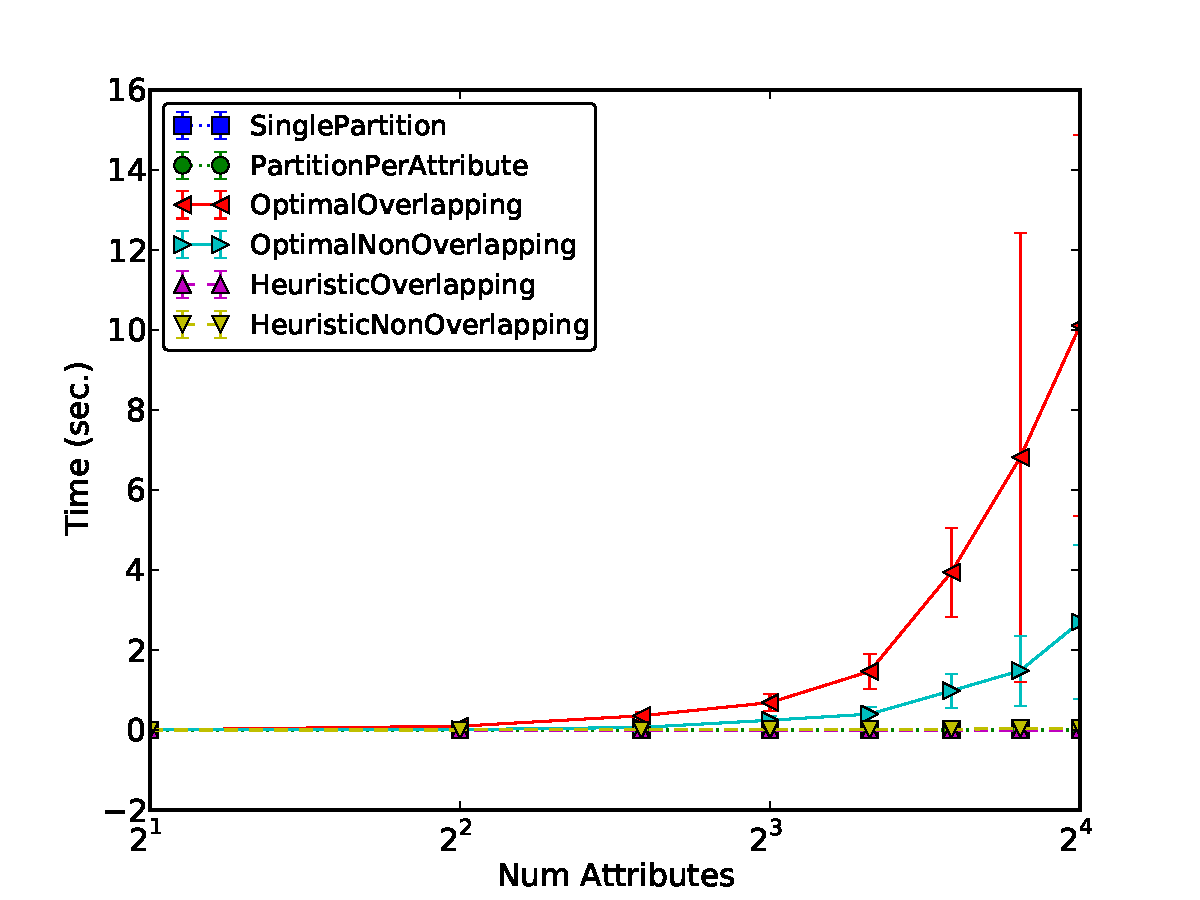
\includegraphics[width=0.33\textwidth]{figures/RunningTimeVsNumAttributes.pdf} &
 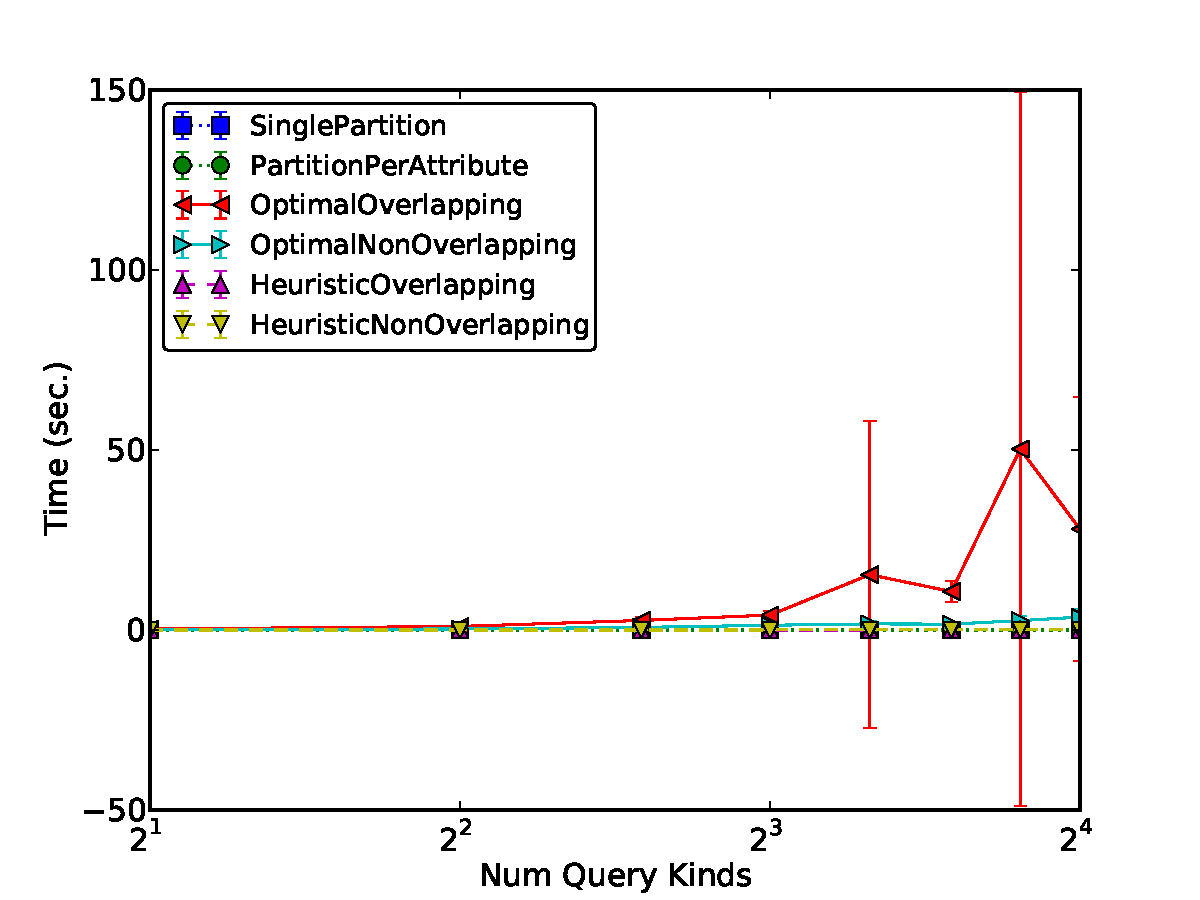
\includegraphics[width=0.33\textwidth]{figures/RunningTimeVsNumQueryKinds.pdf} &
 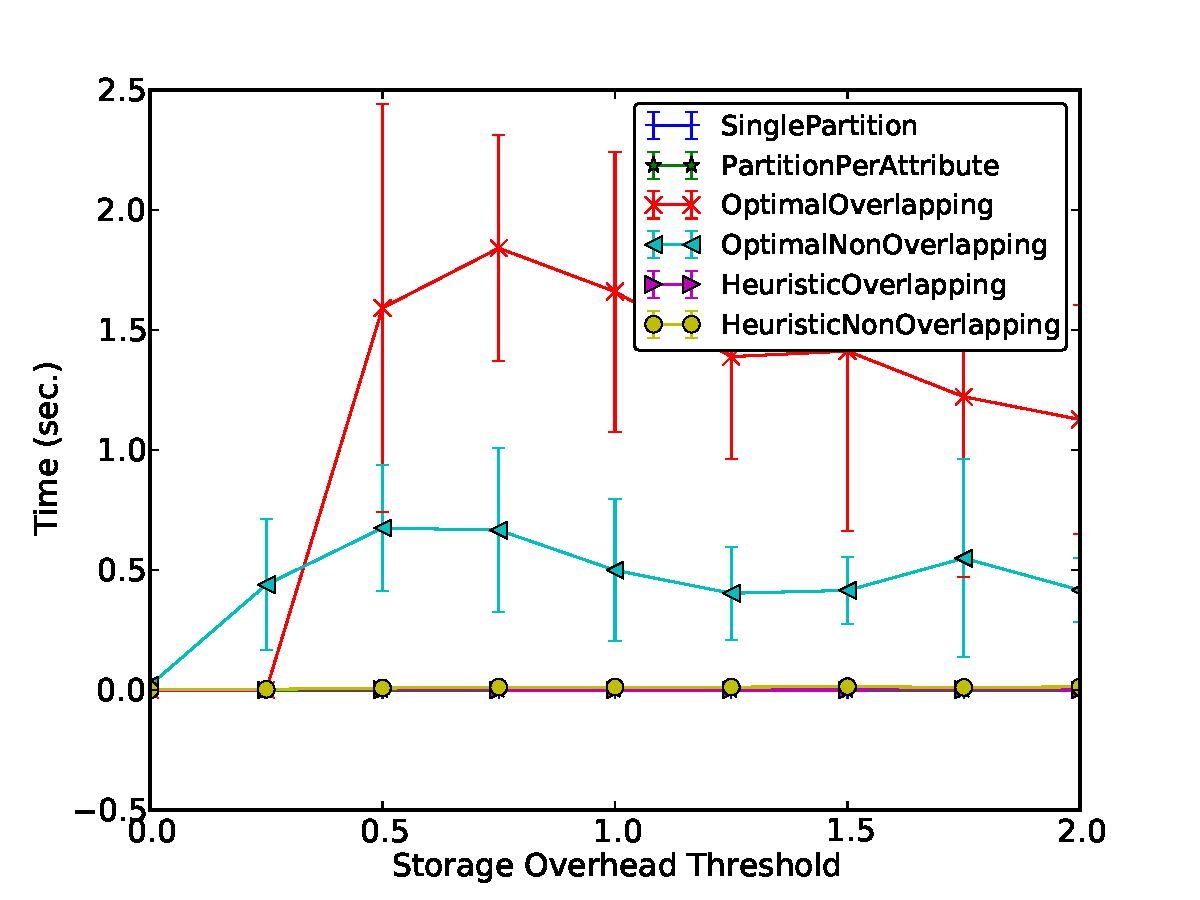
\includegraphics[width=0.33\textwidth]{figures/RunningTimeVsStorageOverheadThreshold.pdf}\\
 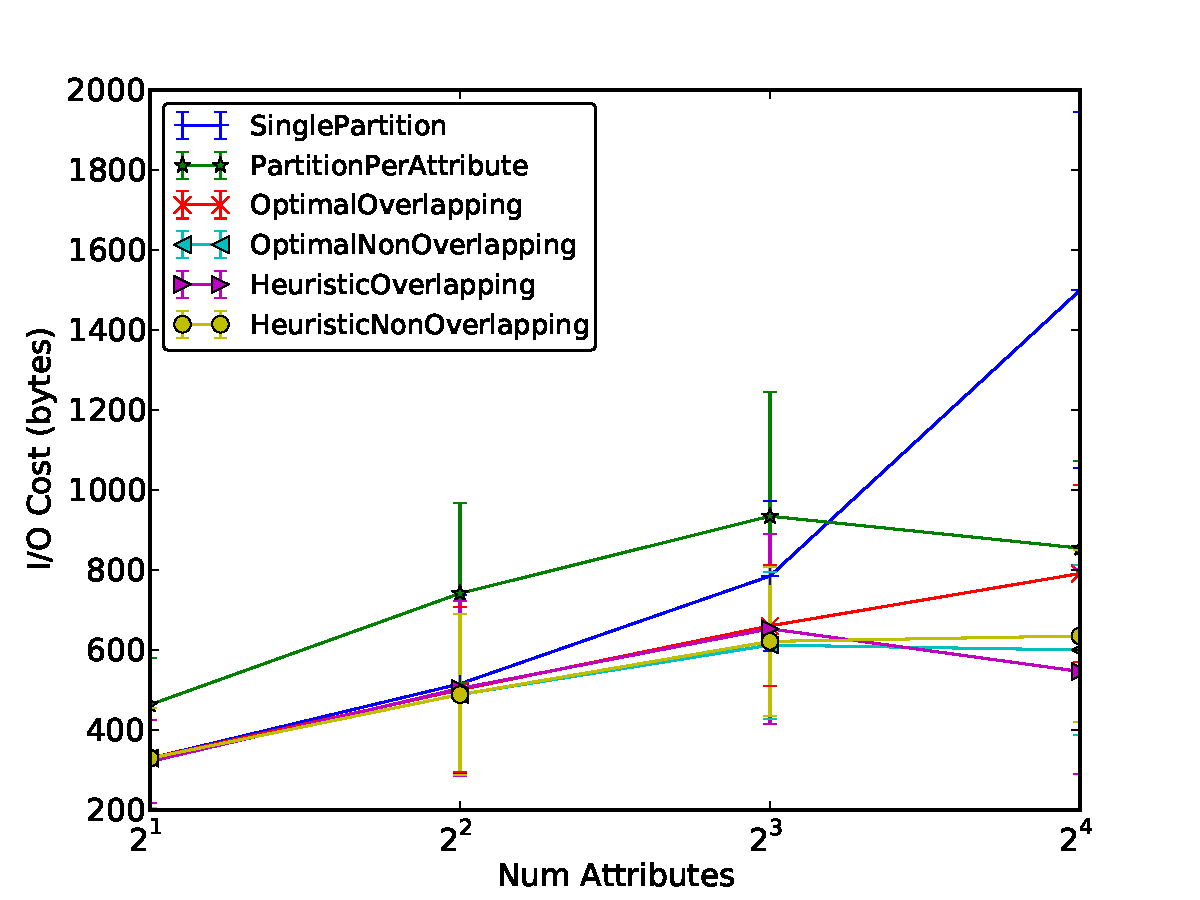
\includegraphics[width=0.33\textwidth]{figures/QueryIOVsNumAttributes.pdf} &
 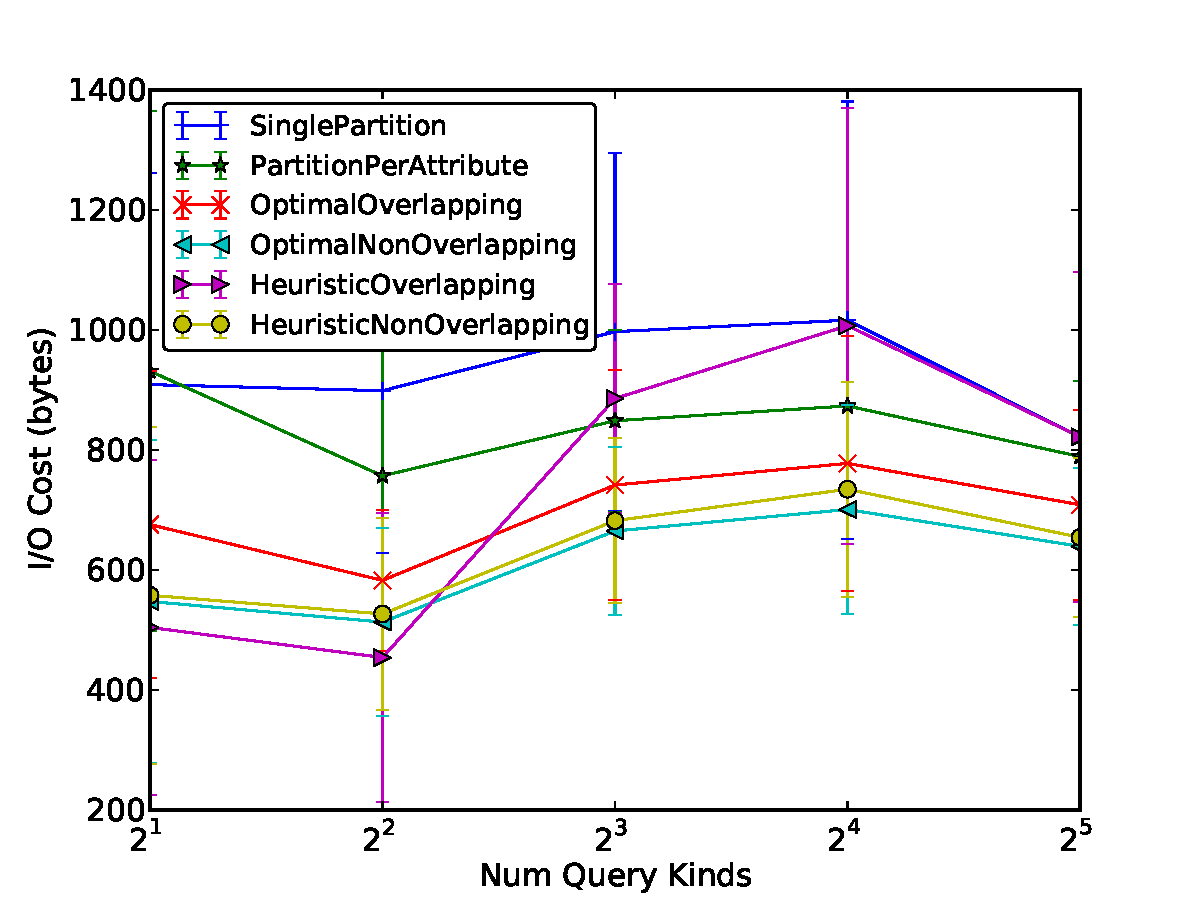
\includegraphics[width=0.33\textwidth]{figures/QueryIOVsNumQueryKinds.pdf} &
 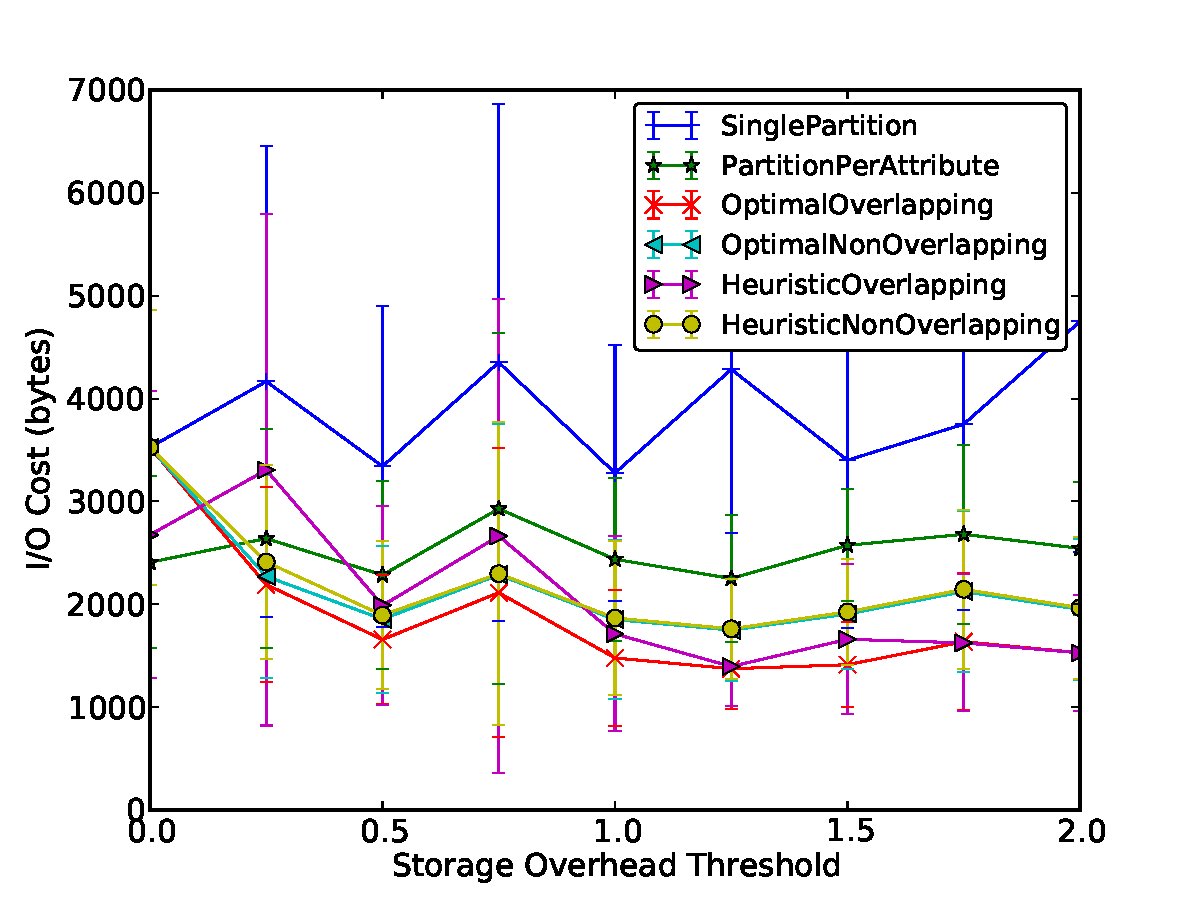
\includegraphics[width=0.33\textwidth]{figures/QueryIOVsStorageOverheadThreshold.pdf}\\
 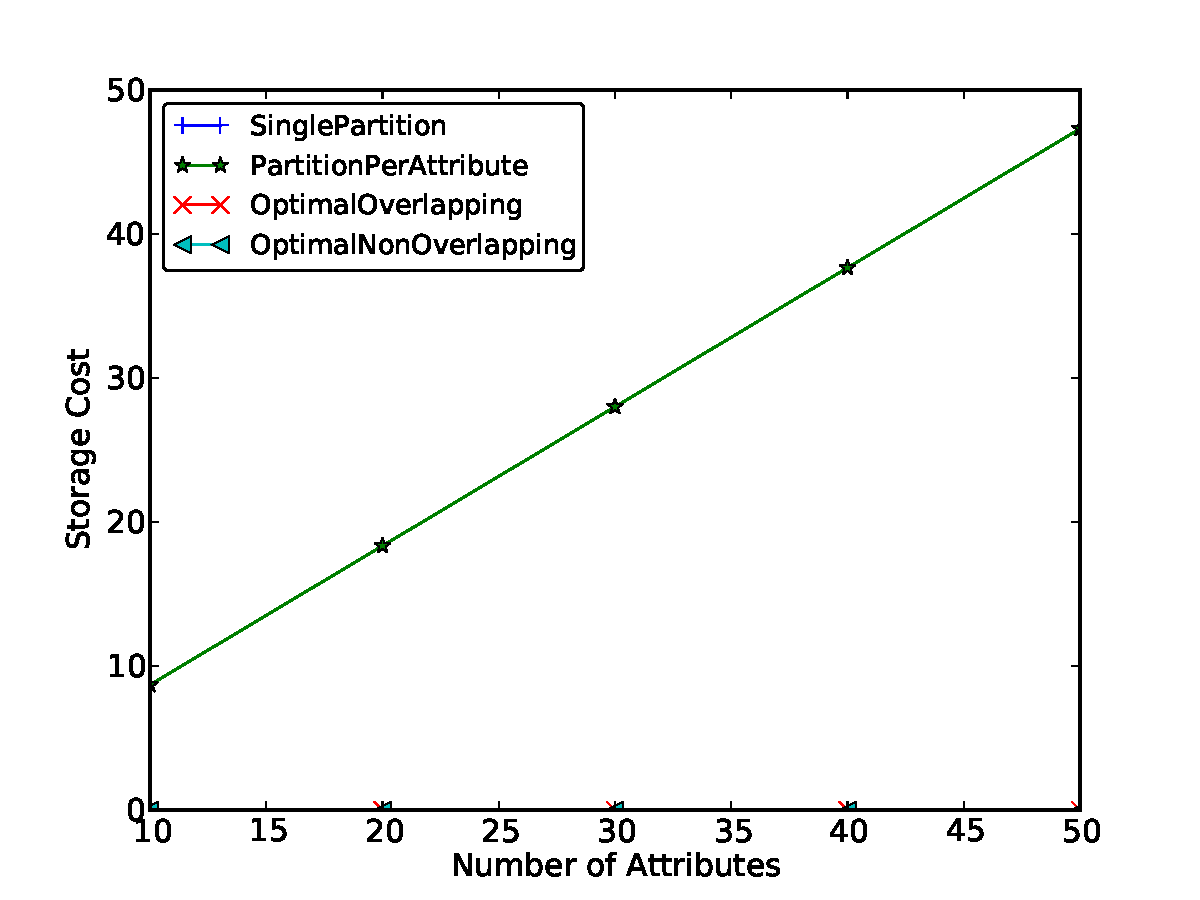
\includegraphics[width=0.33\textwidth]{figures/StorageOverheadVsNumAttributes.pdf} &
 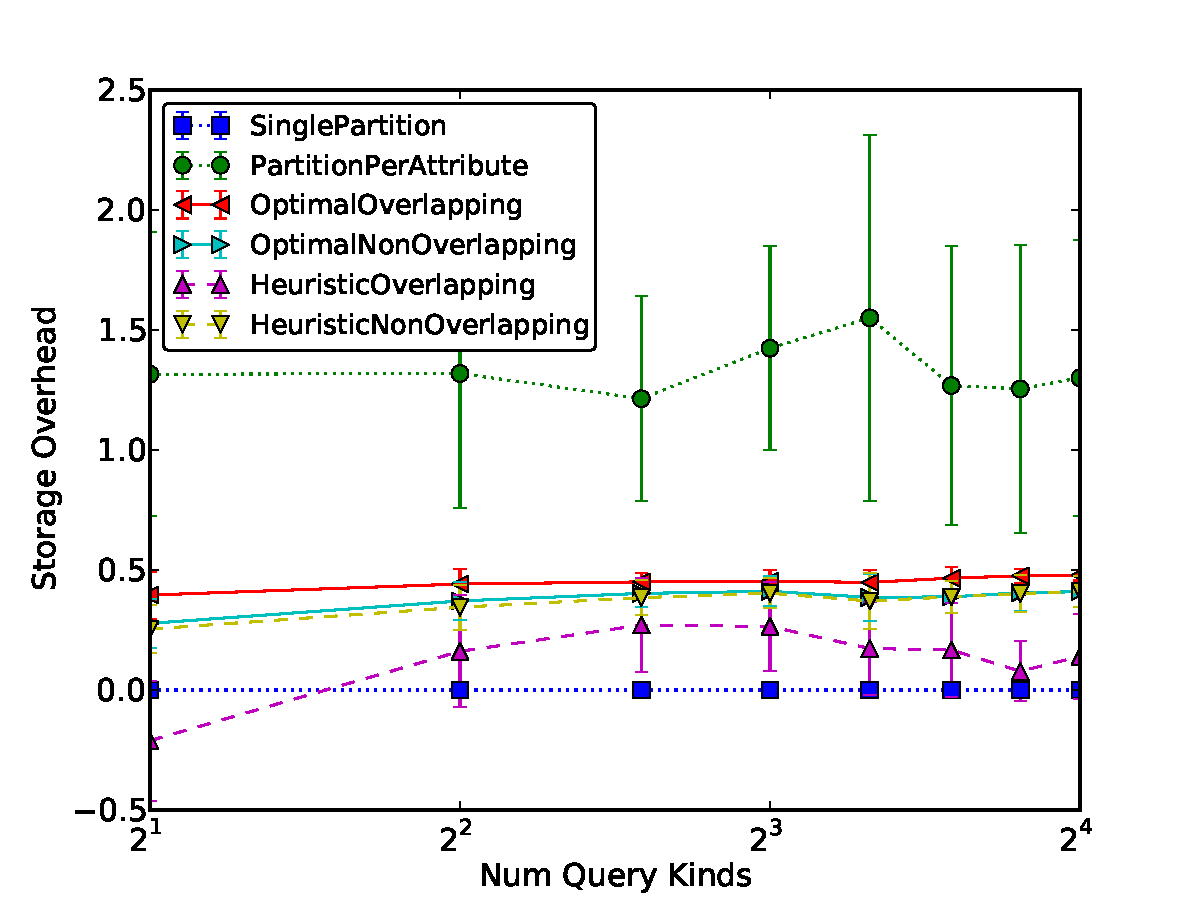
\includegraphics[width=0.33\textwidth]{figures/StorageOverheadVsNumQueryKinds.pdf} &
 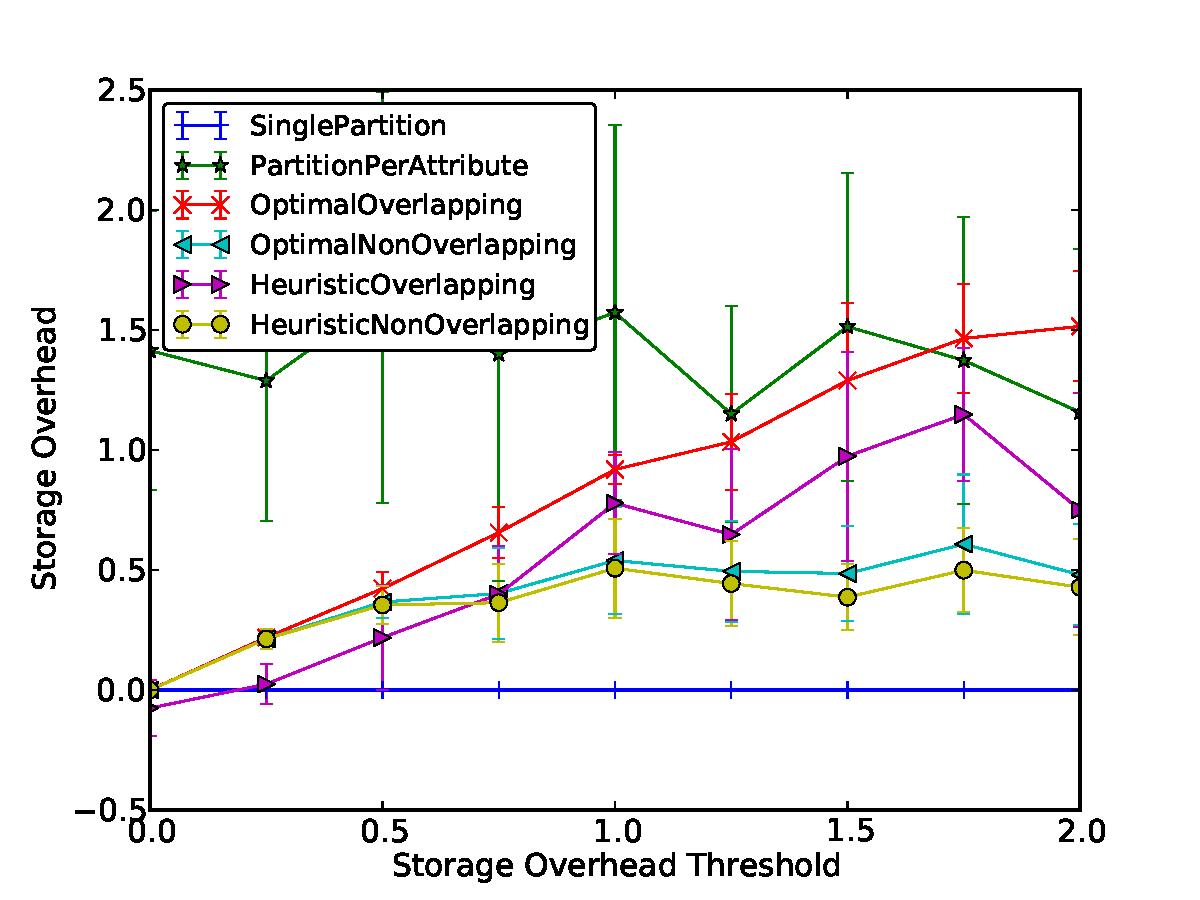
\includegraphics[width=0.33\textwidth]{figures/StorageOverheadVsStorageOverheadThreshold.pdf}\\
 (a)Num Attributes & (b) NumQueryKind &
 (c) StorageOverheadThreshold \\
 \end{tabular}}
\vspace*{1mm}
 \caption{Running time, QueryIO, and StorageOverhead.}
 \label{fig:results}
 \end{figure*}


\section{Related Work}

\begin{alltt}\scriptsize
Gedik et al.~\cite{gedik14}
H2O \cite{alagiannis14}
HYRISE~\cite{grund10}
Bornea et al.~\cite{bornea13}
\end{alltt}


\bibliographystyle{abbrv}
\bibliography{paper}  
\end{document}
